% Created 2019-06-11 mar. 13:30
\documentclass{article}
\usepackage[utf8]{inputenc}
\usepackage[T1]{fontenc}
\usepackage{fixltx2e}
\usepackage{graphicx}
\usepackage{longtable}
\usepackage{float}
\usepackage{wrapfig}
\usepackage{rotating}
\usepackage[normalem]{ulem}
\usepackage{amsmath}
\usepackage{textcomp}
\usepackage{marvosym}
\usepackage{wasysym}
\usepackage{amssymb}
\usepackage{hyperref}
\tolerance=1000
\usepackage[frenchb]{babel}
\author{Valentin LEBOUVIER}
\date{\today}
\title{TP1 : Graphes et Behaviour Trees}
\hypersetup{
  pdfkeywords={},
  pdfsubject={},
  pdfcreator={Emacs 25.2.2 (Org mode 8.2.10)}}
\begin{document}

\maketitle


\section{Présentation Tkinter}
\label{sec-1}
Tkinter est un outil de représentation graphique facile a prendre en main et disponible dans la librairie standard Python.

Présentation Application (Tk)

Présentation Widgets(Button,Canvas)


\section{Ma première fenêtre}
\label{sec-2}
Pour créer votre première fenêtre, il vous suffit d'importer tkinter avec la commande:
\begin{verbatim}
import tkinter as tk
\end{verbatim}

Il vous suffit alors de créer une nouvelle application en créant un objet de type \verb~tk.Tk~ et de le lancer avec la méthode \verb~.mainloop()~.

\noindent
/!$\backslash$ Prenez bien note de lancer la \verb~.mainloop~ en dernier, car il est bloquant.


\noindent
Vous pouvez ensuite commencer a modifier les paramètres de la fenêtre
\begin{itemize}
\item \verb~.title(str)~ : Change le titre de la fenêtre
\item \verb~.geometry(str)~ : Change la taille de la fenêtre et son emplacement sur l'écran
\end{itemize}
\noindent
Pour tout renseignements supplémentaires vous pouvez utiliser \verb~help()~ dans la console.

\section{Les Boutons}
\label{sec-3}
Les boutons \ldots{}. (Création d'un bouton, link vers une fonction/action)

\section{Les canvas}
\label{sec-4}
Les canvas servent principalement a contenir des dessins. Chaque élément du Canvas pourra ensuite être déplacé dans le Canvas.

Pour dessiner dans le canvas vous pouvez utiliser les commandes suivantes:
\begin{itemize}
\item \verb~create_arc()~
\item \verb~create_line()~
\item \verb~create_oval()~
\item \verb~create_rectangle()~
\item \verb~create_polygon()~
\end{itemize}

La plupart de ces fonction demandent la zone dans laquelle la forme doit être dessinée. Les informations demandées sont les point en haut a gauche (\verb~x0~, \verb~y0~) et le point en bas à droite (\verb~x1~, \verb~y1~).

\noindent
/!$\backslash$ Le point en haut à gauche de la fenêtre est le (0,0)


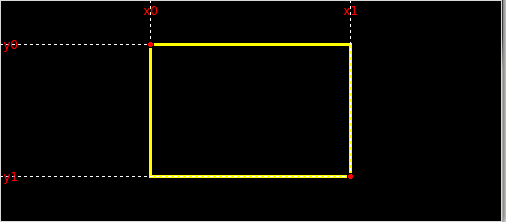
\includegraphics[width=.9\linewidth]{./img/coord_canvas.png}

(Mise en place d'un apercu de jeu de dame avec qqes instructions)
% Emacs 25.2.2 (Org mode 8.2.10)
\end{document}